\documentclass{beamer}
\usetheme{me} % aalto theme


% Packages for math, language, encoding etc.
\usepackage{tikz, ctable}
\usepackage{bm}
\usepackage[finnish]{babel}
\usepackage[utf8]{inputenc}
\usepackage{graphicx}
\usepackage{xcolor}
\usepackage[absolute,overlay]{textpos}	
\usepackage{amsfonts,amssymb,amsbsy,amsthm,amsmath,mathtools,enumerate,verbatim}
\usepackage{stmaryrd} % double square brackets
\usepackage{color, colortbl}
\usepackage[font=scriptsize]{caption}
\usepackage{csquotes}
\usepackage{tabularray}
\usepackage{hyperref}
\usepackage{datetime}

% Theorem defs
\newtheorem{teoreema}{Lause}
\newtheorem{epateoreema}{Epämuodollinen lause}
\newtheorem{määritelmä}{Määritelmä}

% Notation
\DeclareMathOperator{\var}{Var}
\DeclareMathOperator{\n}{\mathrm N}

% Bibliography and style.
\usepackage[style=authoryear]{biblatex}
\addbibresource{sources.bib}
\setbeamertemplate{bibliography item}{}

%\usepackage[
%  backend=biber,
%  style=authoryear,
%]{biblatex}
%\addbibresource{sources.bib}

% Show greyed table of contents before section.
\AtBeginSection[]
{
    \begin{frame}
        \frametitle{Table of Contents}
        \tableofcontents[currentsection]
    \end{frame}
}
\setcounter{tocdepth}{1}


\AtBeginSubsection[]{
  \begin{frame}
  \vfill
  \centering
  \begin{beamercolorbox}[sep=8pt,center,shadow=true,rounded=true]{subtitle}
    \usebeamerfont{subtitle}\insertsubsectionhead\par%
  \end{beamercolorbox}
  \vfill
  \end{frame}
}

% Info about presentation
\title{Keskeinen raja-arvolause ja sen sovellukset liiketoiminnassa}
%\subtitle{}
%\author{Jaakko Pere}

\newdate{date}{25}{3}{2025}
\date{\displaydate{date}}


% Page number
%\setbeamertemplate{footline}[frame number]

%%%%%%%%%%%%%%%%%%%%%%%%%%%%%%%%%%%%%%%%%%%%%%%%%%%%%%%%%%%%%%%%%%%%%%%%%%%%%%%
%%%%%%%%%%%%%%%%%%%%%%%%%%%%%%% DOCUMENT BEGINS %%%%%%%%%%%%%%%%%%%%%%%%%%%%%%%
%%%%%%%%%%%%%%%%%%%%%%%%%%%%%%%%%%%%%%%%%%%%%%%%%%%%%%%%%%%%%%%%%%%%%%%%%%%%%%%
\begin{document}

\frame{\titlepage}

\begin{frame}{Agenda of the presentation}
\tableofcontents
\end{frame}

%%%%%%%%%%%%%%%%%%%%%%%%%%%%%%%%%%%

\begin{frame}{Kohdeyleisö}
  \begin{itemize}
    \item Ensimmäisen ja toisen vuoden kandiopiskelijat
  \end{itemize}
\end{frame}

%%%%%%%%%%%%%%%%%%%%%%%%%%%%%%%%%%%

\begin{frame}{Moraali}
  \begin{itemize}
    \item Suurten lukujen laki
  \end{itemize}
\end{frame}

%%%%%%%%%%%%%%%%%%%%%%%%%%%%%%%%%%%

\begin{frame}{Opetustavoitteet}
  Luennon jälkeen
  \begin{enumerate}
    \item osaamme approksimoida todennäköisyyksiä klassisen keskeisen raja-arvo
    lauseen avulla,
  \end{enumerate}
\end{frame}

%%%%%%%%%%%%%%%%%%%%%%%%%%%%%%%%%%%



%%%%%%%%%%%%%%%%%%%%%%%%%%%%%%%%%%%

\section{Lyhyt kertaus: Suurten lukujen laki}

%%%%%%%%%%%%%%%%%%%%%%%%%%%%%%%%%%%

\section{Normaalijakauma}

\begin{frame}
  Normaalijakauma on absoluuttisesti jatkuva jakauma. Merkitsemme
  normaalijakaumaa parametrein $\mu\in(-\infty, \infty)$ ja
  $\sigma^2\in(0,\infty)$ notaatiolla $\n\left(\mu, \sigma^2\right)$. Jakauman
  $\n\left(\mu, \sigma^2\right)$ tiheysfunktio on
  \begin{equation*}
    f(x) = \frac{1}{\sqrt{2\pi\sigma^2}} e^{-\frac{\left(x-\mu\right)^2}
    {2\sigma^2}}.
  \end{equation*}
  \pause
  \begin{itemize}
    \item[]
  \end{itemize}
  Tällöin normaalijakauman kertymäfunktio voidaan esittää tiheysfunktion avulla
  \begin{equation*}
    F\left(x\right) = \int_{-\infty}^{x} f(t)\,\mathrm{d}t
  \end{equation*}
\end{frame}

%%%%%%%%%%%%%%%%%%%%%%%%%%%%%%%%%%%

\begin{frame}
  \begin{center}
    \begin{figure}
      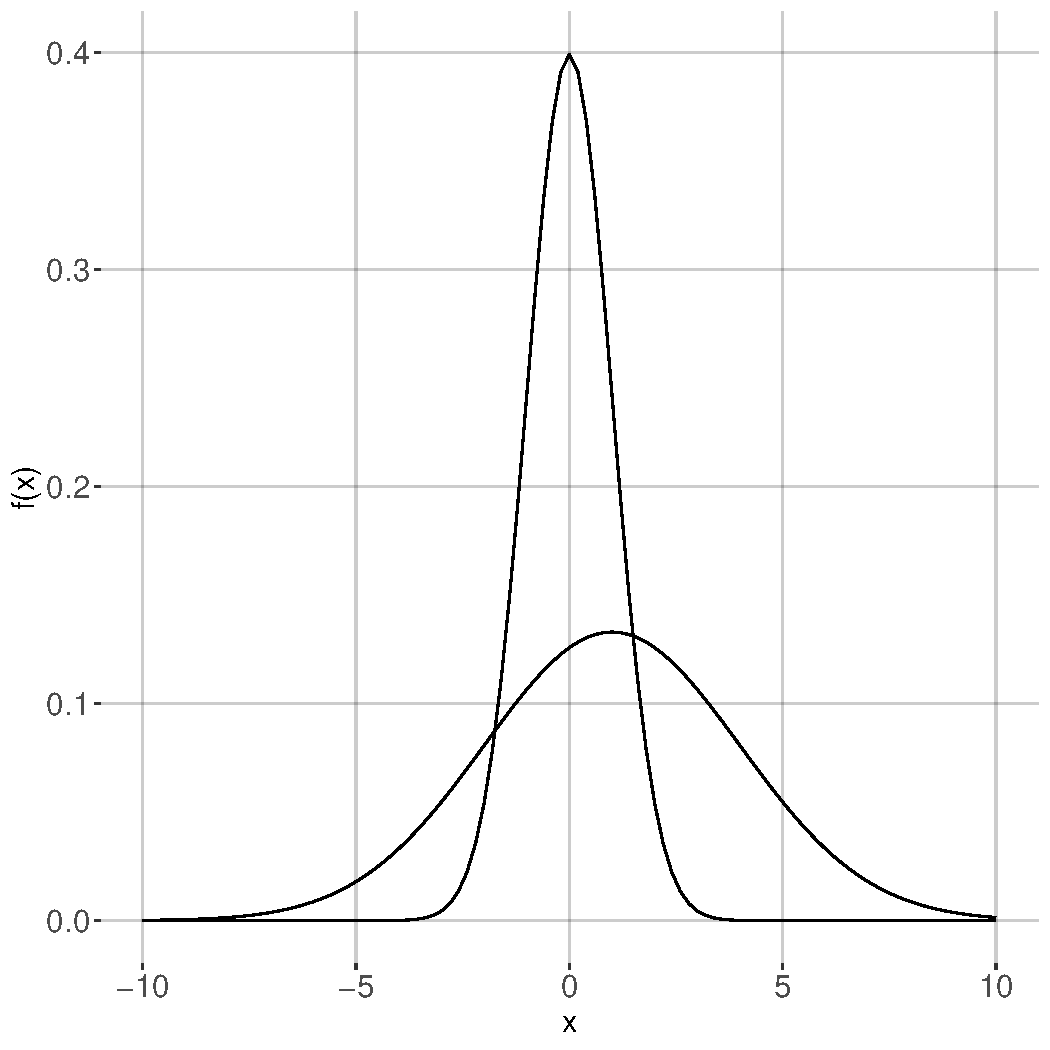
\includegraphics[width=0.7\textwidth, height=0.7\textwidth]{normal}
      \caption{Normaalijakaumat $\n\left(0,1\right)$ (katkoviiva) ja $\n\left(1, 9\right)$ (jatkuva viiva).}
  \end{figure}
\end{center}
\end{frame}

%%%%%%%%%%%%%%%%%%%%%%%%%%%%%%%%%%%

\section{Keskeinen raja-arvolause}

%%%%%%%%%%%%%%%%%%%%%%%%%%%%%%%%%%%

\begin{frame}
  \begin{teoreema}
    Olkoon $X_1, X_2, \ldots, X_n$ riippumattomia ja samoin jakautuneita
    satunnaismuuttujia niin, että $\mathbb{E}\left(\left|X_1\right|^2\right) <
    \infty$. Merkitsemme $\bar X = \frac{1}{n}\sum_{i = 1}^n X_i$, $\mu =
    \mathbb{E}\left(X_1\right)$ ja $\sigma = \sqrt{\var\left(X_1\right)}$.
    Tällöin, kun otoskoko $n$ on suuri,
    \begin{equation*}
      \tilde X = \sqrt{n}\frac{\bar X - \mu}{\sigma}
    \end{equation*}
    noudattaa likimain standardinormaalijakaumaa $\n\left(0, 1\right)$,
    \pause
    \begin{equation*}
      \mathbb{P}\left(\tilde X \leq x\right) \approx
      \int_{-\infty}^x \frac{1}{\sqrt{2\pi}}e^{-t^2/2}\,\mathrm{d}t.
    \end{equation*}
  \end{teoreema}
\end{frame}

%%%%%%%%%%%%%%%%%%%%%%%%%%%%%%%%%%%

%%%%%%%%%%%%%%%%%%%%%%%%%%%%%%%%%%%

\begin{frame}{Intuitio}
  Toisin sanoen kun otoskoko $n$ on suuri, niin $\bar X$ noudattaa likimain
  jakaumaa
  \begin{equation*}
    \n\left(\mu, \frac{\sigma^2}{n}\right).
  \end{equation*}
\end{frame}

%%%%%%%%%%%%%%%%%%%%%%%%%%%%%%%%%%%

\begin{frame}{Kurssin ulkopuolista asiaa}
  \begin{itemize}
    \item 
  \end{itemize}
\end{frame}

%%%%%%%%%%%%%%%%%%%%%%%%%%%%%%%%%%%

\section{Sovellukset}

\subsection{Sovellus 1: Todennäköisyyksien approksimointi}

\subsection{Sovellus 2: Luottamusväli}

\begin{frame}{Tiivistelmä}
  
\end{frame}

\begin{frame}[allowframebreaks]{Lähdeluettelo}
  \printbibliography
\end{frame}
\end{document}
